Each network was tested with ten different thresholds against 52 CT images using the metrics described in chapter \ref{Experiment}. For the sake of simplicity, the results from the 52 CT images are taken as a mean in figure \ref{fig:MeanValues}.
\begin{figure*}
        \centering
        \begin{subfigure}[b]{0.475\textwidth}
            \centering
            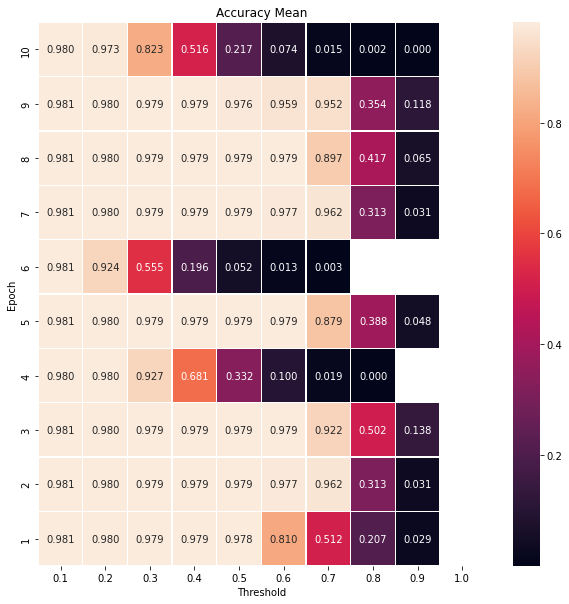
\includegraphics[width=\textwidth]{PICs/accuracy_mean.png}
            \caption[Accuracy Mean]%
            {{\small Accuracy Mean}}    
            \label{fig:acMean}
        \end{subfigure}
        \hfill
        \begin{subfigure}[b]{0.475\textwidth}  
            \centering 
            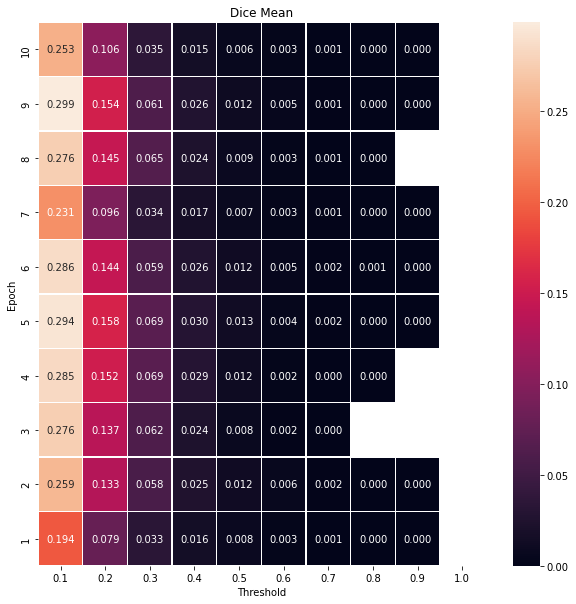
\includegraphics[width=\textwidth]{PICs/dice_mean.png}
            \caption[Dice Coefficient Mean]%
            {{\small Dice Coefficient Mean}}    
            \label{fig:diceMean}
        \end{subfigure}
        \vskip\baselineskip
        \begin{subfigure}[b]{0.475\textwidth}   
            \centering 
            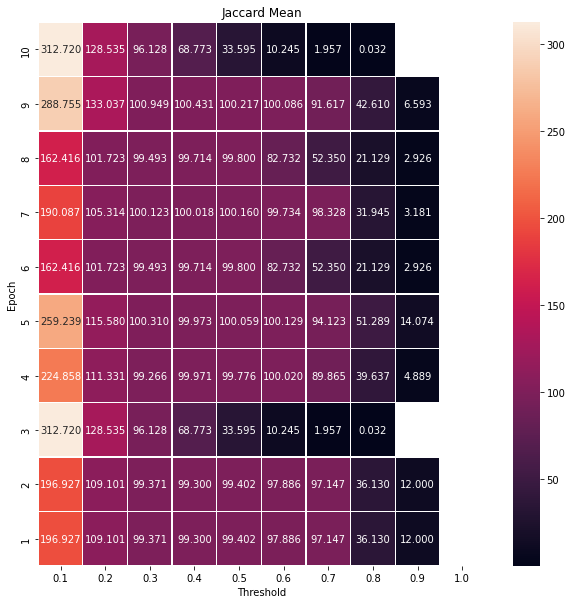
\includegraphics[width=\textwidth]{PICs/jaccard_mean.png}
            \caption[Jaccard Index Mean]%
            {{\small Jaccard Index Mean}}    
            \label{fig:jMean}
        \end{subfigure}
        \hfill
        \begin{subfigure}[b]{0.475\textwidth}   
            \centering 
            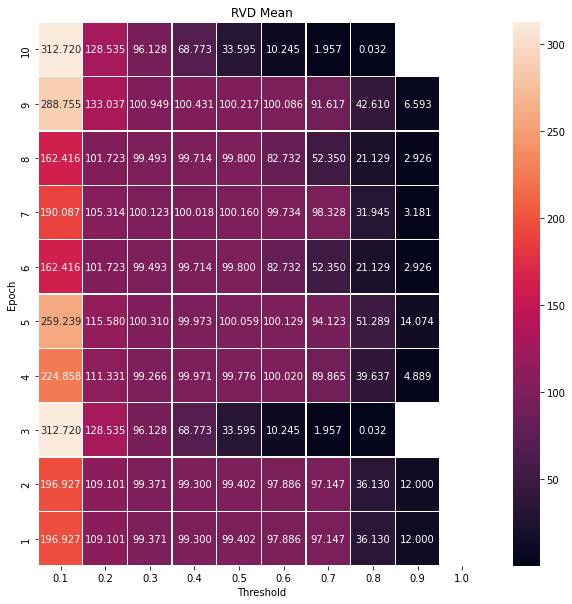
\includegraphics[width=\textwidth]{PICs/rvd_mean.png}
            \caption[RVD Mean]%
            {{\small RVD Mean}}    
            \label{fig:rvdMean}
        \end{subfigure}
        \caption[ Mean Average, Dice Coefficient, Jaccard Index and RVD for each epoch from one to ten and threshold 0.1 to 1.0 ]
        {\small Mean Average, Dice Coefficient, Jaccard Index and RVD for each epoch from one to ten and threshold 0.1 to 1.0} 
        \label{fig:MeanValues}
    \end{figure*}
    
The results displayed in figure \ref{fig:MeanValues} indicate greater results on a lower threshold, which deteriorate as the threshold increases. The performance drops significantly when the threshold reaches 0.5. Noticeably, the \ac{DSC} performs worse than the accuracy. This indicates a large unbalance between the amount of background and kidney pixels. An example can be seen in figure \ref{fig:kidneyMask}, where the green prediction mask is more than twice the size of the pink ground truth is more than double in size. Additionally, the kidney is also small, compared to the rest of the background.

 \begin{figure}
 \centering
 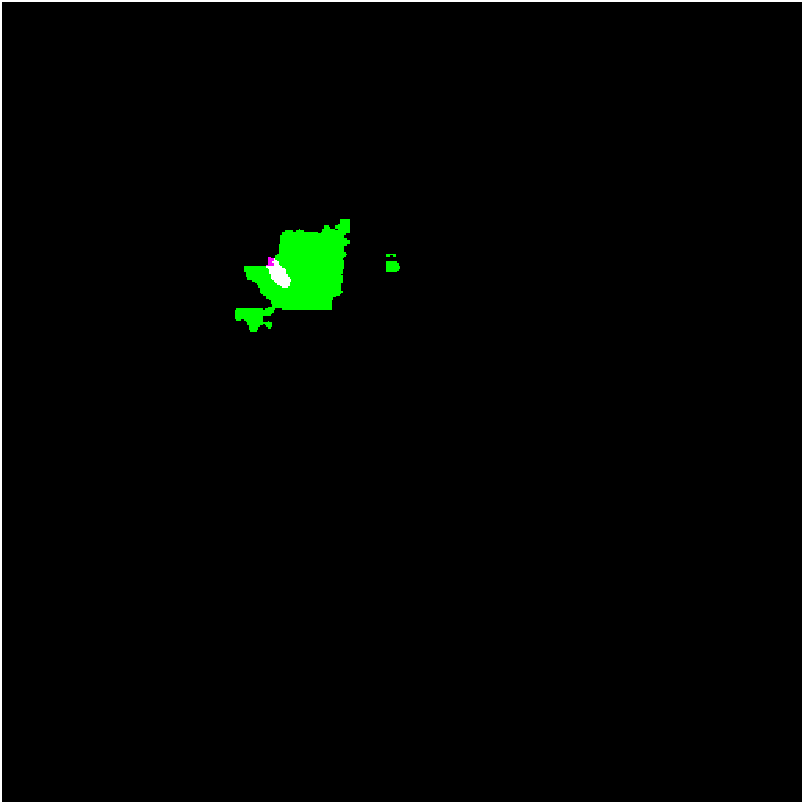
\includegraphics[width=0.3\linewidth]{PICs/kidneyMask.png}
 \caption{Prediction over ground truth label - Pink: kidney label; Green: prediction mask}
 \label{fig:kidneyMask}
 \end{figure}
 
 
For further analyzation, results using the network of epoch five and an 0.5 threshold were grouped by CT image and taken as a mean, in order to display  the performance of  the model for the different parts of the kidney (see figure \ref{fig:align}).
 \begin{figure}
 \centering
 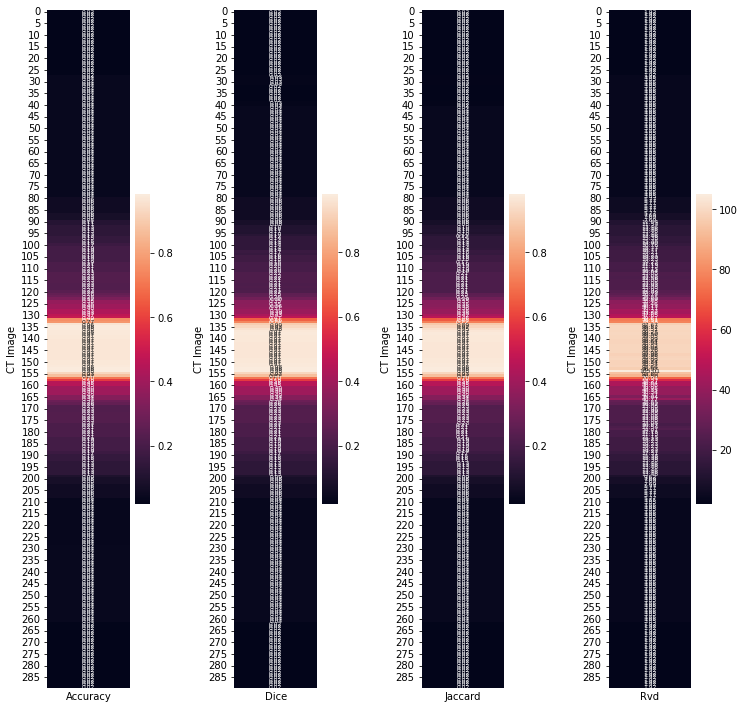
\includegraphics[width=0.5\linewidth]{PICs/align.png}
 \caption{Epoch: 5, Threshold: 0.5 - Mean  Accuracy, Jaccard Index, Dice Coefficient and RVD from top to bottom}
 \label{fig:align}
 \end{figure}
 
 The volume distribution can be seen in figure \ref{fig:volumeDistribution}. Details are attached at the end of the thesis.
 \begin{figure}[!htbp]
 \centering
 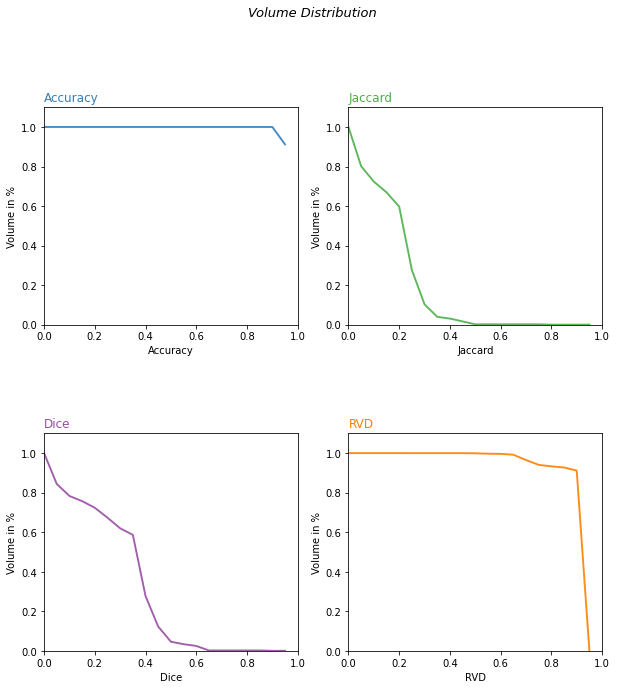
\includegraphics[width=0.9\linewidth]{PICs/volumeDistibution.png}
 \caption{Volume Distribution for Accuracy, Jaccard Index, Dice Coefficient and RVD  - epoch 5, threshold 0.5, RVD $10^{-2}$ }
 \label{fig:volumeDistribution}
 \end{figure}
\ac{J}, \ac{DSC} and \ac{RVD} in figure \ref{fig:volumeDistribution} show low performance while \ac{AC} being the only positive indicator. \ac{J} and \ac{DSC} display low congruence with the expert segmentation while \ac{RVD} indicate large differences between prediction and actual segmentation. The visualization of figure \ref{fig:align} clearly shows a better performance in the middle part of the kidney, where it has a more regular and balanced form than at the top or bottom, where unbalanced data is to be expected. This leads to the conclusion, that Mask R-CNN is able to segment objects of a class if the form and size does not change but fails if otherwise. In regards to the research questions, it can be concluded that it is not feasible to train Mask R-CNN for automated kidney segmentation because of the low congruence with expert segmentation. With a segmentation time of approximately 0.1254 seconds per slice or 6.4464 seconds per CT image, the model is fast enough for practical usage, but based on the other metrics, it is not advised. 
%Limitation 
Nevertheless, this conclusion is based on the given data and the usage of a 2D Mask R-CNN implementation of Matlab \cite{GitHub.25Aug22, .25Aug22}. Although papers as "\citetitle{Vuola.29Jan19}" \cite{Vuola.29Jan19}  and   \citetitle{OvergaardLauersen.2021} \cite{OvergaardLauersen.2021} display the shortcomings of Mask R-CNN with organic images and describe tasks such as kidney segmentation as challenging, different papers suggest better results or improvements. As an example, in \citetitle{Goyal.2022} \cite{Goyal.2022} the framework reaches a \ac{DSC} of 90,5\% and a \ac{J} of 82,8 \%, while other papers \cite{Chen., Shu.2020} reach metrics significantly above 90\%  by developing the framework even further. 
One of the suggested developments was the change from a two dimensional ROI Align to a three dimensional ROI Align algorithm. Another paper, \citetitle{Nazari.2021} \cite{Nazari.2021}, uses a similar approach to reach a better performance.  Even though the aggregated results indicate low performance, they also show high \ac{AC} with low \ac{DSC}. This is typical for unbalance data as described above. This supports the theory for the need of further research by improving the current framework.